\documentclass{article}                     % onecolumn (standard format)

\usepackage{graphicx}
\usepackage{float}
\usepackage{amsmath}
\usepackage{cite}
\usepackage{subfig}
\usepackage{rotating}
\usepackage[left=2.2cm, right=2.2cm]{geometry}
\usepackage{algpseudocode}
\usepackage{algorithm}
%\floatstyle{ruled}
\usepackage{hyperref}
\usepackage{algpseudocode}
\usepackage{tikz}
\usetikzlibrary{positioning,calc,shapes,shapes.geometric}
\usepackage{pgf}
\usepackage{verbatim}
\newfloat{algorithm}{tbp}{loa}
\providecommand{\algorithmname}{Algorithm}
\floatname{algorithm}{\protect\algorithmname}
%
% \usepackage{mathptmx}      % use Times fonts if available on your TeX system
%
% insert here the call for the packages your document requires
%\usepackage{latexsym}
% etc.
%
% please place your own definitions here and don't use \def but
% \newcommand{}{}
%

%
\begin{document}
	
\title{Introduction to AI - assignment 5}


\author{Oded~Yechiel         \and
	Matan~Rusanovsky
}

\date{3/1/19}

\maketitle

\section{Introduction}
	In this assignment we provide a Sequential decision making under uncertainty using belief-state MDP for decision making.
	A utility table is kept by the agent to decide how to act based on the current state in order to achieve the maximum expected performance.
	

\section{Construction of a state and a utility table}
The state of the agent can be viewed as a tuple consisted from:
\begin{enumerate}
	\item the location of the agent
	\item the remaining time
	\item the amount of people saved
	\item the amount of people in the vehicle
	\item for each vertex containing people a Boolean value stating if the people were picked up already or not
	\item for each edge a three value variable stating if the edge is blocked, clear or unknown
\end{enumerate}

For this program, using Python provides a huge advantage in that there is built-in hushing of tuples, so constructing a table based on the state tuple is extremely easy and state forward.

The table is initialized (Algorithm~\ref{alg:tabinit}) by iterating through all of the permutation possible for the state and providing a 0 utility value. In order to avoid unnecessary computation, unfeasible states are discarded from the table. 

For example, suppose there is one vertex containing 2 people and one vertex containing 1 people. A feasible state could be that there are 2 people in the vehicle and the number of saved people is $ \leq 1 $. Another feasible state could be that there is 2 person saved and in the vehicle there are $ \leq 1 $ in the vehicle. However, it is unfeasible that there are 2 people in the vehicle and 2 people saved. This sort of state is ignored. 

\begin{algorithm}
	\caption{Table initialization}
	\label{alg:tabinit}		
	\begin{algorithmic}[1]
		\Procedure{InitUtility}{Graph}
		\State Utility $ \leftarrow  $ dict()
		\For     {each state permutation in the Graph}
		\If     {state is Feasible}
		\State  Utility[state] = 0
		\EndIf
		\EndFor
		\State \Return Utility
		\EndProcedure
	\end{algorithmic}
\end{algorithm}

Once the table is initialized, value iteration is performed on the utility table for $ N $ iterations, or until convergence. 

\section{Decision making using utility table}
The 
\begin{algorithm}
	\caption{Act based on utility table}
	\label{alg:dm}		
	\begin{algorithmic}[1]
		\Procedure{ActBasedUtility}{State, Utility}
		\State $ BestActionValue \leftarrow -\infty $
		\State $ BestAction \leftarrow -1 $  //stay in place
		\For     {each Action in possible actions}
		\State $ NewState \leftarrow \textsc{StateFromAction(State, Action)} $
		\If     {$ Utility[NewState] > BestActionValue $}
		\State  $ BestActionValue \leftarrow Utility[NewState]$
		\State  $ BestAction \leftarrow Action$
		\EndIf
		\EndFor
		\State \Return $ BestAction $
		\EndProcedure
	\end{algorithmic}
\end{algorithm}

\section{Run example}
\subsection{First example}
In this example we run a simple graph with different blockage probability between vertex 1 and vertex 2.
\begin{figure}
	\centering
	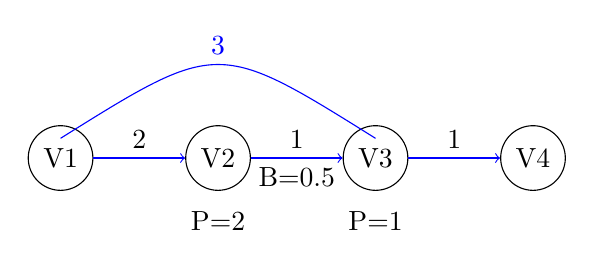
\begin{tikzpicture}
	\node [draw, circle] (V1) at (0, 0) {V1};
	\node [draw, circle] (V2) at (2, 0) {V2};
	\node [draw=none] (V2p) at (2, -0.8) {P=2};
	\node [draw, circle] (V3) at (4, 0) {V3};
	\node [draw=none] (V1p) at (4, -0.8) {P=1};	
	\node [draw, circle] (V4) at (6, 0) {V4};		
	\path [draw=blue, ->] (V1) -- (V2) node[midway, anchor=south]{2};
	\path [draw=blue, ->] (V2) -- (V3) node[midway, anchor=south]{1} node[midway, anchor=north]{B=0.5};
	\path [draw=blue, ->] (V3) -- (V4) node[midway, anchor=south]{1};		
 	\draw[blue] (0,0.25) .. controls(2, 1.5) .. (4, 0.25) node[midway, anchor=south]{3};
	
	\end{tikzpicture}
	\caption{Example graph}
	\label{fig:bn2}
\end{figure}
\subsubsection{Input}
\begin{verbatim}
file: "input2.txt"

#V 4          ; number of vertices n in graph (from 1 to n)
#V 1 Ev 2
#V 2 Ev 1

#E1 0 1 2 
#E2 1 2 1 B 0.5
#E3 2 3 1 
#E4 0 2 3


#Deadline 5
#Start 0
#Shelter 3
\end{verbatim}

\subsubsection{Output}
This simple example elegantly demonstrates the different policy that will be chosen based on the blockage probability. Since the deadline is 5, a single person can be saved for sure if the agent will go from V1 to V3 to V4, taking 4 time to cross. However, the agent can go from V1 to V2 and hope there will be no blockage and continue to the shelter and save all people. However, if there is a blockage the agent will not be able to save anyone.

The blockage probability value has a huge impact on the agent's decision. If the blockage probability  is smaller than $ 2/3 $ the agent will take a chance on saving everyone since the utility for going to V1 is
$$ U[V1] = (1 - P(B))\times 3000 + P(B) \times 0 $$
As opposed to going to V3 where the utility is 1000.

The output for 0.5 can be seen below for a random run:
\begin{verbatim}
Edge 0: V0(0) <-> V1(2) --- W=2, P_blockage=0.0, Blocked=False
Edge 1: V1(2) <-> V2(1) --- W=1, P_blockage=0.5, Blocked=True
Edge 2: V2(1) <-> V3(0) --- W=1, P_blockage=0.0, Blocked=False
Edge 3: V0(0) <-> V2(1) --- W=3, P_blockage=0.0, Blocked=False

Starting value iteration for 200 Epochs
Finished value iteration after 194 Epochs
(@0, 0IV, 0Sav, 5[T], 1500.0[U])
(@1, 2IV, 0Sav, 3[T], 0.0[U])
(@0, 2IV, 0Sav, 1[T], 0.0[U])
(@1, 2IV, 0Sav, 0[T], 0[U])
\end{verbatim}
As seen above, the agent took a chance and lost due to blockage.

\subsection{Second example}
For the same example above but with no blockage the output will look as follows:
\begin{verbatim}
Edge 0: V0(0) <-> V1(2) --- W=2, P_blockage=0.0, Blocked=False
Edge 1: V1(2) <-> V2(1) --- W=1, P_blockage=0.5, Blocked=False
Edge 2: V2(1) <-> V3(0) --- W=1, P_blockage=0.0, Blocked=False
Edge 3: V0(0) <-> V2(1) --- W=3, P_blockage=0.0, Blocked=False

Starting value iteration for 200 Epochs
Finished value iteration after 194 Epochs
(@0, 0IV, 0Sav, 5[T], 1500.0[U])
(@1, 2IV, 0Sav, 3[T], 3000.0[U])
(@2, 3IV, 0Sav, 2[T], 3000.0[U])
(@3, 0IV, 3Sav, 1[T], 3000.0[U])
(@2, 0IV, 3Sav, 0[T], 3000[U])
\end{verbatim}
In this case the agent was able in saving everyone.

\subsection{Third example}
This example is larger and takes more time to complete. The graph looks as follows
\begin{figure}
	\centering
	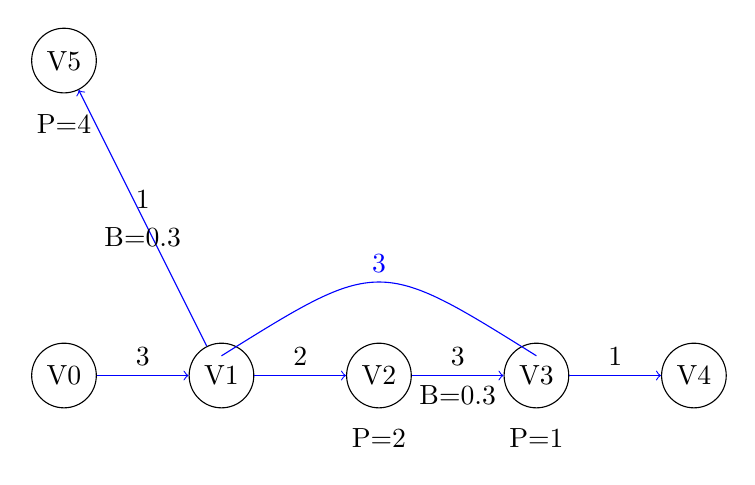
\begin{tikzpicture}
	\node [draw, circle] (V0) at (0, 0) {V0};
	\node [draw, circle] (V1) at (2, 0) {V1};
	\node [draw, circle] (V2) at (4, 0) {V2};
	\node [draw=none] (V2p) at (4, -0.8) {P=2};
	\node [draw, circle] (V3) at (6, 0) {V3};
	\node [draw=none] (V1p) at (6, -0.8) {P=1};	
	\node [draw, circle] (V4) at (8, 0) {V4};		
	\node [draw, circle] (V5) at (0, 4) {V5};
	\node [draw=none] (V5p) at (0, 3.2) {P=4};		
	\path [draw=blue, ->] (V0) -- (V1) node[midway, anchor=south]{3};		
	\path [draw=blue, ->] (V1) -- (V2) node[midway, anchor=south]{2};
	\path [draw=blue, ->] (V2) -- (V3) node[midway, anchor=south]{3} node[midway, anchor=north]{B=0.3};
	\path [draw=blue, ->] (V3) -- (V4) node[midway, anchor=south]{1};		
	\draw[blue] (2,0.25) .. controls(4, 1.5) .. (6, 0.25) node[midway, anchor=south]{3};
	\path [draw=blue, ->] (V1) -- (V5) node[midway, anchor=south]{1} node[midway, anchor=north]{B=0.3};	
	
	\end{tikzpicture}
	\caption{Example graph}
\end{figure}

\subsubsection{Input}
\begin{verbatim}
#V 6          ; number of vertices n in graph (from 1 to n)
#V 2 Ev 2
#V 3 Ev 1
#V 5 Ev 4

#E1 0 1 3 ; Edge1 between vertices 1 and 2, weight 1
#E2 1 2 2 ; Edge2 between vertices 2 and 3, weight 3
#E3 2 3 3 B 0.3; Edge3 between vertices 3 and 4, weight 3
#E6 1 5 1 B 0.3; Edge3 between vertices 3 and 4, weight 3
#E4 1 3 3 ; Edge4 between vertices 2 and 4, weight 4
#E5 3 4 1 ; Edge4 between vertices 2 and 4, weight 4

#Deadline 10
#Start 0
#Shelter 4
\end{verbatim}
\subsubsection{Output}
\begin{verbatim}
Edge 1: V0(0) <-> V1(0) --- W=3, P_blockage=0.0, Blocked=False
Edge 2: V1(0) <-> V2(2) --- W=2, P_blockage=0.0, Blocked=False
Edge 3: V2(2) <-> V3(1) --- W=3, P_blockage=0.3, Blocked=True
Edge 6: V1(0) <-> V5(4) --- W=1, P_blockage=0.3, Blocked=False
Edge 4: V1(0) <-> V3(1) --- W=3, P_blockage=0.0, Blocked=False
Edge 5: V3(1) <-> V4(0) --- W=1, P_blockage=0.0, Blocked=False

Starting value iteration for 200 Epochs
Finished value iteration after 192 Epochs
(@0, 0IV, 0Sav, 10[T], 4130.0[U])
(@1, 0IV, 0Sav, 7[T], 5000.0[U])
(@5, 4IV, 0Sav, 6[T], 5000.0[U])
(@1, 4IV, 0Sav, 5[T], 5000.0[U])
(@3, 5IV, 0Sav, 2[T], 5000.0[U])
(@4, 0IV, 5Sav, 1[T], 5000.0[U])
(@3, 0IV, 5Sav, 0[T], 5000[U])
\end{verbatim}
\end{document}


